\section{SpecBuf}
The side-channel which forms the basis of multiple Spectre variants is the modification of data cache state during speculative execution.
To improve performance, modern out-of-order cores will speculatively fetch data into the core on a load miss.
However, in the event that the load miss is misspeculated, the refill data is still written into the cache, potentially evicting other resident cache lines.
By carefully measuring the execution times of repeated loads, attacker code can inspect the state of the cache and infer the destination addresses of misspeculated loads by the victim code.

To address this issue, the tag and data arrays must be considered as part of the ``architectural state'' of the machine, since their contents will affect the ``architectural'' results of timing measurements performed by attacker code.
Similar to how architectural register state is managed in the execution pipelines of out-of-order machines, a secure core must only allow correctly speculated, committing instructions to modify the cache state.
A proposed approach is to hold speculated load data in an ``L0 Speculation buffer'' that can be flushed when misspeculation is realized.
This prevents misspeculated loads from affecting the state of the cache, while still allowing correctly speculated loads to broadcast their data into the rest of the machine as soon as possible, maintaining performance. If well implemented, such a buffer could slightly improve performance by deferring the eviction of prior contents, slightly reducing the miss latency, and could even be combined with a store coalescing buffer - another useful ``L0 buffer'' structure.

\subsection{Miss Status Holding Registers}
\begin{figure}
  \begin{center}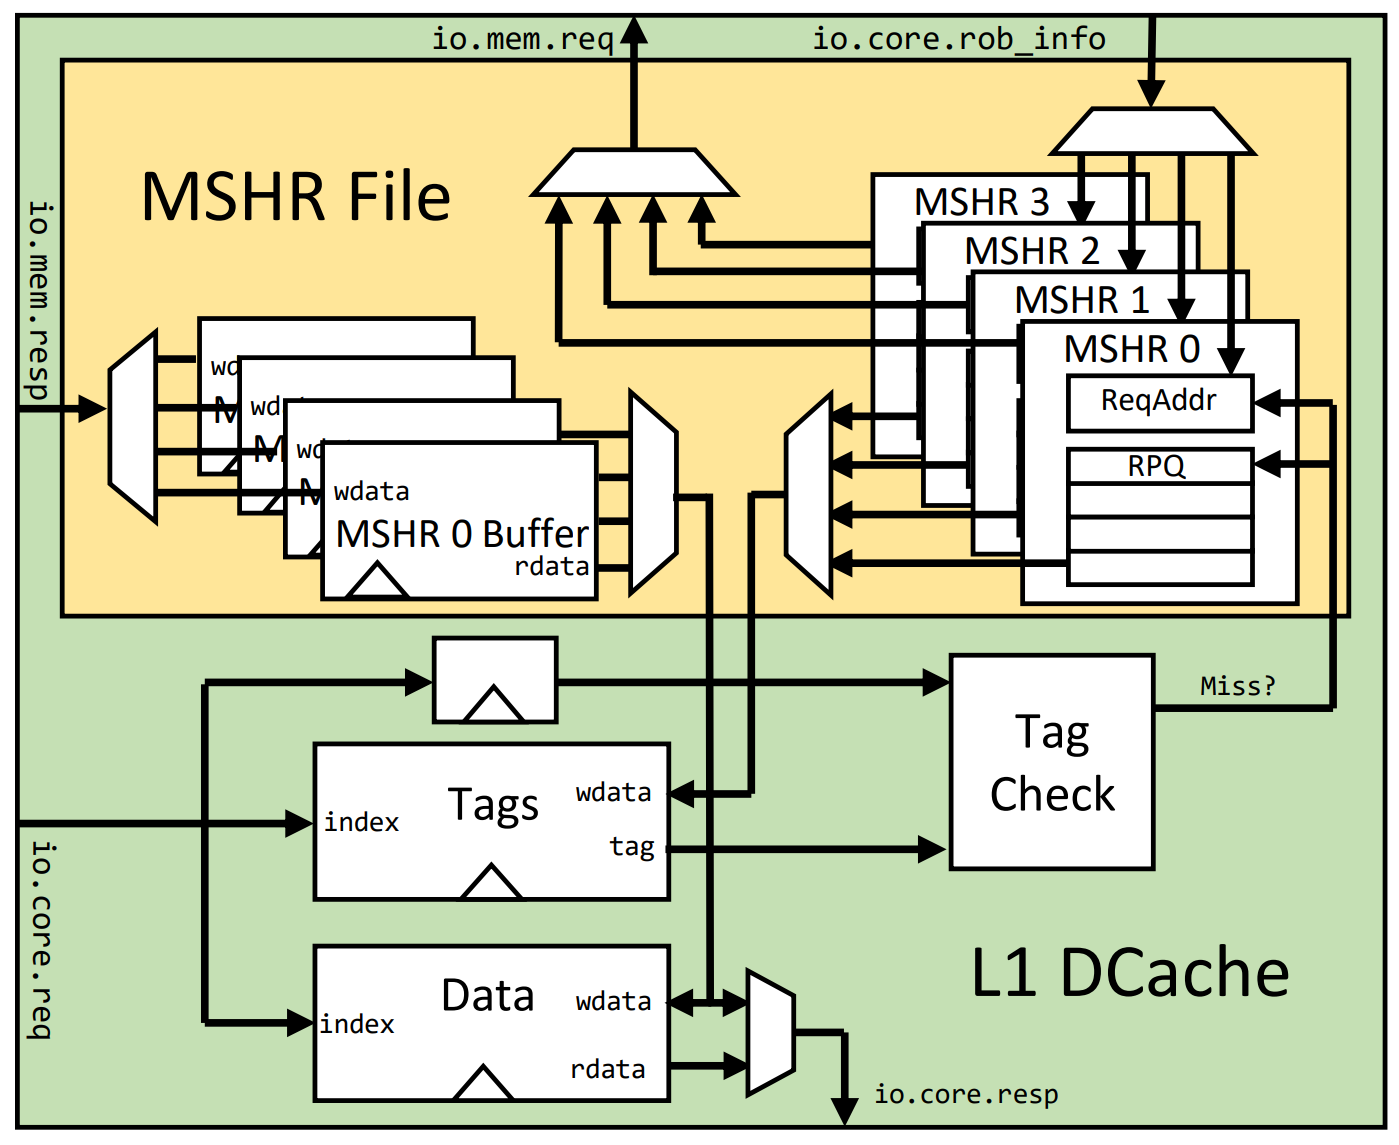
\includegraphics[scale=0.17]{dcache.png}\end{center}
  \caption{Design of modified L1 data cache}
\end{figure}

We implement such a speculation buffer as part of the Miss Status Holding Registers (MSHRs) in BOOM's L1 data cache. The MSHRs hold the status of inflight memory requests made by the L1 cache to the L2 memory bus.
In the original data cache, L2 cache refills would write the refill data into the tag and data arrays before waking up the corresponding MSHRs to return the load data to the core.
To implement a speculation buffer, we modified cache refills to instead write the refill data into per-MSHR cacheline buffers.

On misspeculation, the misspeculated MSHR entry is flushed along with any load data that has been returned. Only after the load which allocated the MSHR entry is known to be committed is the new cacheline written into the tag and data arrays. This effectively prevents misspeculated loads from altering the state of the cache.

Since speculating past loads is necessary for performance, we allow bypassing request data out of the speculation buffer, before the data is committed into the tag and data arrays. The consequence of this bypassing is that the service time for a cache miss is unchanged from the original behavior.

Another subtlety of the MSHRs is the per-MSHR replay queues, which hold subsequent requests to the same cache-line. These queues are necessary for handling consecutive load misses to the same cacheline without occupying more valuable MSHR entries. Our speculation buffer will eagerly empty the replay queues until a store miss is seen in the queue. Since stores issued to the memory system are always non-speculative, the cacheline can be immediately committed.

\subsection{MSHR Optimization}


\subsection{Point of No Return}
In the naive implementation of the speculation buffer, entries in the buffer are only deallocated when the instruction is reached by the head of the reorder buffer (ROB). However, this can result in heavy MSHR utilization, since there may be many instructions between a waiting load and the commit head waiting to execute and write back. However, we observe that many of those instructions, while still inflight, can be marked as guaranteed to commit.

This leads to the concept of a ``point-of-no-return'' (PnR) in the ROB, in addition to the commit head. While the commit head tracks the next instruction which will commit the architectural state, the PnR tracks instructions which are guaranteed to eventually commit, even if they have not yet completed execution. In other words, the PnR points at the oldest instruction which may cause misspeculated execution; an unsafe instruction, such as a branch which has not yet executed. If an instruction is marked as safe, the PnR will pass it whether or not it has completed executing. We observe that refills in the spec-buffer can be committed to the cache as soon as the PnR passes the instruction which triggered them. This reduces pressure on MSHR resources and prevents backpressure on incoming cache requests.

To reduce the performance impacts of our speculation buffer, we implemented a PnR in the ROB. Two versions were implemented. The first simple-PnR is a less expensive pointer that will only mark at most one ROB row per cycle as ``guaranteed to commit''. We also implemented a more complex PnR head that can mark an arbitrary number of rows per cycle, essentially ``jumping over'' groups of safe instructions to the oldest instruction unsafe.
